\section{Results}

\subsection{Population density and tweeting location}

The distribution of tweets over the municipalities is visualized on Figure \ref{all_tweet_map}. On Figure \ref{heat_map} we show a heatmap of twitter activity for only one month (over the whole dataset this was too computation intensive). From these maps show that indeed highly populated areas have higher twitter activity. However, our question was more subtle, we were interested if the 


\begin{figure}[h]
  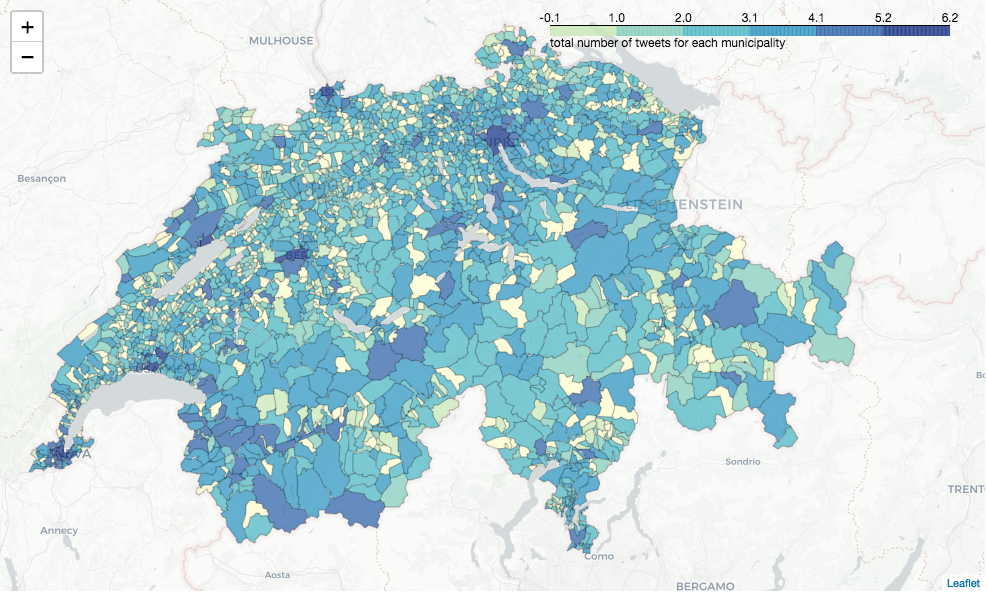
\includegraphics[width=0.5\textwidth]{images/all_tweet_map.png}
  \caption{Colors on the map show the logarithm (base 10) of the number of tweets in the whole dataset coming from each municipality}
  \label{all_tweet_map}
\end{figure}



\begin{figure}[h]
  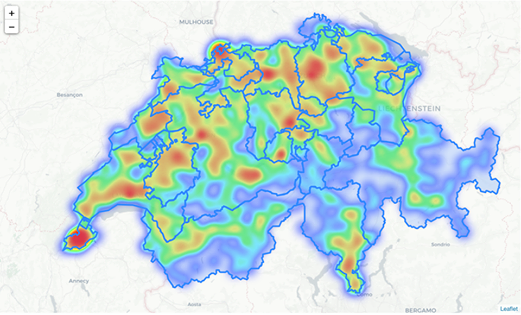
\includegraphics[width=0.5\textwidth]{images/heat_map.png}
  \caption{The heatmap of the number of tweets in September 2016.}
  \label{heat_map}
\end{figure}


\subsection{Reconstructing the R\"ostigraben}
Figure \ref{rosti_map}

\begin{figure}[h]
  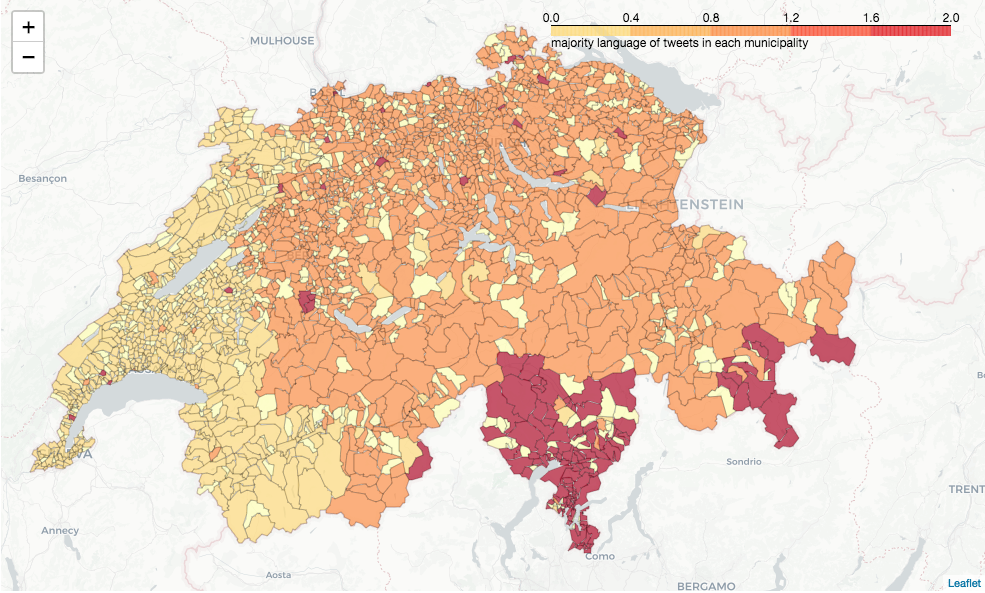
\includegraphics[width=0.5\textwidth]{images/rosti_map.png}
  \caption{The R\"ostigraben reconstructed from the language of the tweets. The color encoding is yellow: French; orange: German, red: Italian}
  \label{rosti_map}
\end{figure}


\subsection{Political activity}

TODO: Ramtin 
